\chapter{Literature Review} \label{literature}
In this chapter we will present different energy trading models proposed in literature
and their limitations. On each of the presented models, we will focus on two different
aspects:
\begin{itemize}
    \item \textbf{The market layer}: It comprises the market's allocation and payment rules and defines
          a clear biding mechanism. Its main purpose is to allocate the available traded energy based on the
          the bids of energy buyers and sellers. It defines how the market is getting cleared.
    \item \textbf{The blockchain/information layer}: It connects all market participant and provide the market platform with equal
          access to everyone in the microgrid, to avoid discrimination. It's integrated with the market layer to ensure
          data security and privacy. In the following chapters different blockchain technologies, used on P2P energy trading, will
          be presented. \cite{DeTrade,BrooklynMicrogrid}
\end{itemize}


\section{A Hyperledger Fabric Implementation}
\label{sec:hfi}
In this section we will describe a P2P energy trading platform proposed by M. Pipattanasomporn et al \cite{Pipattanasomporn2013}.
This study focuses mainly on the blockchain layer implementation and uses a simplistic market clearing method.
It focuses mainly on photovoltaic (PV) energy trading and makes use of the open-source Hyperledger Fabric blockchain framework
to implement a private blockchain.
\subsection{Market Layer}
The proposed energy market is split in time periods of an hour. Each hour, network peers submit their buy and sell
bids for energy that will be traded the next hour. The market clearing is done based on the market clearing price (MCP).
The MCP used for this study was the average bid price of the buyers:
\begin{center}
    \begin{math}
        MCP_t = \frac{\sum_{i=1}^{N_t} \beta_{n,t} \times kWh_{n,t}}{\sum_{i=1}^{N_t} kWh_{n,t}}
    \end{math}
\end{center}
Where,\\
\begin{tabular}{rl}
    $MCP_t$       & :  Market clearing price                                     \\
    $\beta_{n,t}$ & :  Bid of buyer $n$ at hour $t$ (token/kWh)                  \\
    $kWh_{n,t}$   & :  Number of kWhs to be purchased from buyer $n$ at hour $t$ \\
    $N$           & :  Total number of buyers                                    \\
\end{tabular}\\
The matching of buying and selling bids are done with the first-in, first-out approach (FIFO) and priority is given to
buying offers with the highest value ($\beta_{n,t}\times kWh_{n,t}$). The market is cleared every hour $t$ using the
$MCP_t$, calculated with the formula above. \cite{Pipattanasomporn2013}

\subsection{Blockchain Layer}
For the blockchain layer, a private blockchain network approach is used. Each participant need to register and be
authorized to use the energy trading network. For the registration, the participant need to provide their first
and last name, their email which acts also as a unique identifier of the participant and their initial balance in
the token/currency used for energy exchange. A certificate authority is responsible to register new identities and
issue enrolment certificates for participants.\\
In this design, two type of assets and four type of transactions are defined.\\
\textbf{\underline{Assets}}:
\begin{itemize}
    \item The \textbf{PV} asset: Each participant that has a PV and wants to sell their excess energy generation,
          need to register their PV unit as an asset in the blockchain. This asset contains a unique identifier for the
          PV unit and the identifier of the participant owning the unit.
    \item The \textbf{kWhlisting} asset: It is automatically generated by the system every hour and contains a
          listing id, a state, a list of all the selling offers and another one for the buying offers. The listing id
          consists of the date and time when the asset created and the state defines the state of the listing which can
          either be at the state of accepting offers from buyers and sellers or at auction closed state where the auction
          stops. In simple terms, this asset gathers all the buying and selling bids for a specific hour.
    \item Energy generation and consumption needs should be known ahead of time. The energy trading negotiations are
          done one hour before the actual energy generation and consumption. This could lead in surplus energy that was not
          consumed or required energy that was not produced.
\end{itemize}
\textbf{\underline{Transactions}}:
\begin{itemize}
    \item The "\textbf{AcceptOfferBroadcast}" transaction: It is automatically send by the system to
          all network participant at the start of each hour, to inform them that they can start bidding.
    \item The "\textbf{PVOffer}" transaction: After receiving the 'AcceptOfferBroadcast' transaction,
          each participant that owns a PV unit can send this transaction to define how much excess energy they
          want to trade (kWh) and what is their reserve price (token).
    \item The "\textbf{BUYOffer}" transaction: Once receiving the 'AcceptOfferBroadcast' message, all
          participants can send the "BUYOffer" transaction, to define the amount of energy they need (kWh) along
          with the price (token/kWh) they want to pay.
    \item The "\textbf{CloseBidding}" transaction: It is automatically send by the system at the end
          of each hour to inform the participants that the bidding is closed and the market clearing process
          initiated.
\end{itemize}
\begin{figure}[h!]
    \centering
    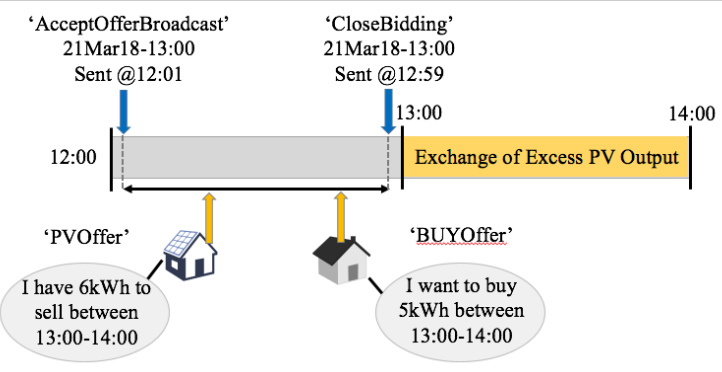
\includegraphics[scale=0.4]{Figures/transaction_timeline.png}
    \caption{Transaction timeline proposed by M. Pipattanasomporn et al \cite{Pipattanasomporn2013}}
\end{figure}
The market clearing process is encoded in a smart contract code that is embedded in the "CloseBidding"
transaction. When this transaction is executed the smart contract code is executed and the market is
cleared as described in the market layer section above.
\cite{Pipattanasomporn2013}

\subsection{Limitations}
This design has some limitations that need to be considered:
\begin{itemize}
    \item The way the market is designed in hourly intervals, doesn't allow for inter-temporal commitments. This means that only energy needs of the next our can be covered
          and no energy trading planning for different time periods could be made.
    \item The market clearing price algorithm is very simplistic, alternative approaches need to be explored
    \item Prosumers might not be truthful about their hour ahead energy production or the forecasting might have some errors. This can lead to violations to the energy trading
          commitments. Such a system couldn't be self sustained, it needs to be connected to the grid to cover any extra energy needs.
\end{itemize}

\section{DeTrade and DeMarket}
\label{sec:dtr}
DeTrade is a decentralized P2P energy trading platform proposed by Ayman Esmat et al \cite{DeTrade}. It allows the energy trading participants to trade energy among them, while guarantying privacy
and security of their identities and market bids. It makes use of novel P2P energy trading market called DeMarket which is described in more detail in the \textbf{Market Layer}
subsection below.\\
In the proposed design, a, AI smart agent is assigned to each network peer. This AI agent has the following responsibilities:
\begin{itemize}
    \item Monitors the energy consumption and production of the peer by having access directly to the smart meters.
    \item Makes bids in the DeMarket
    \item Clears the market
    \item Makes Contact with the blockchain layer
\end{itemize}
The market results are stored safely and immutably on the blockchain layer after it is cleared. A smart contract is also implemented on the blockchain layer that makes sure the money
are transferred only if the energy was really traded. The smart contract is the contact point between the market and the blockchain layers.
\cite{DeTrade}

\begin{figure}[h!]
    \centering
    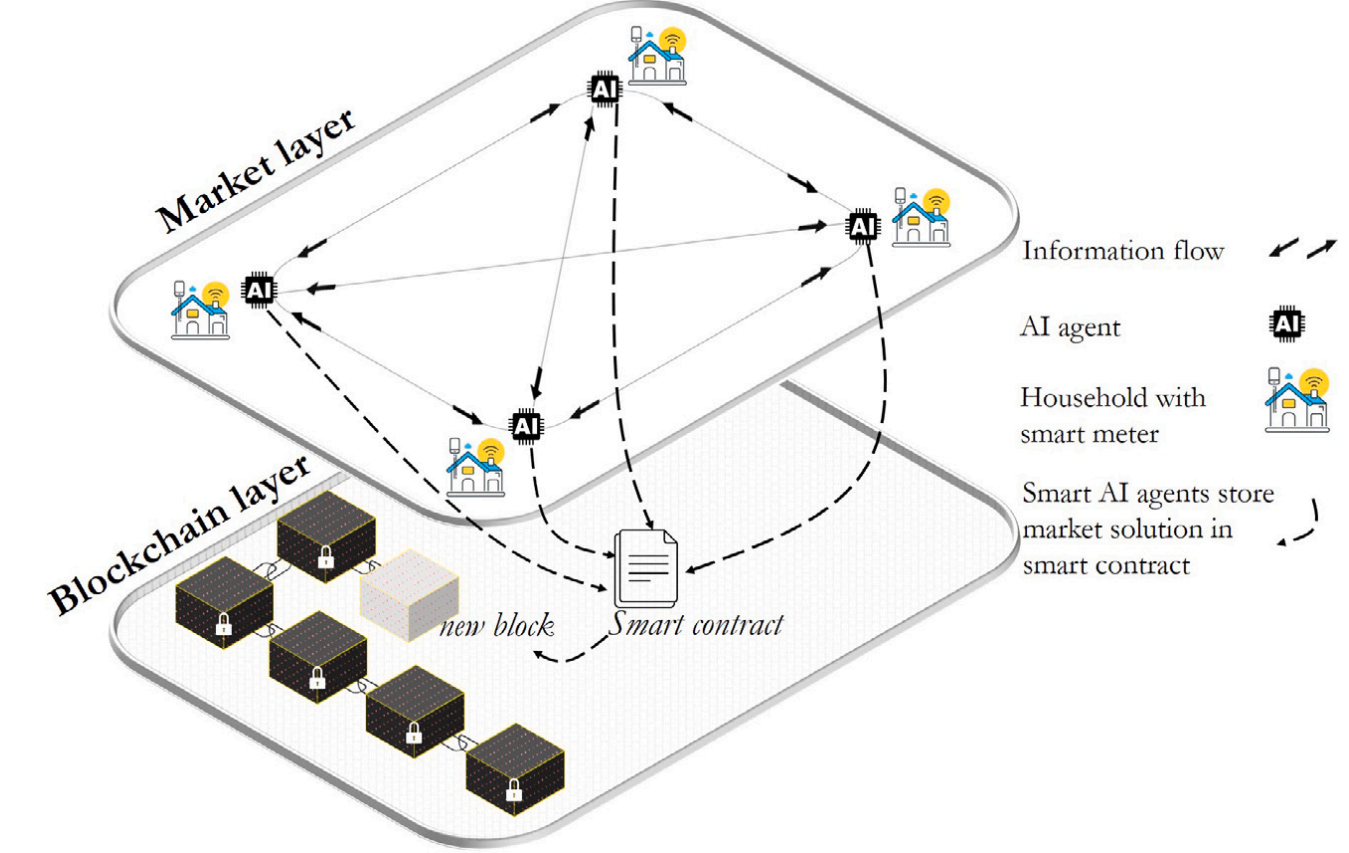
\includegraphics[scale=0.3]{Figures/DeTrade.png}
    \caption{DeTrade Architecture \cite{DeTrade}}
\end{figure}

\subsection{Market Layer - DeMarket}
DeMarket is a short-term parallel pool-based market that allows market participants to trade various market products. It has an uniform pricing mechanism and is divided in multiple
periods of market clearing and energy delivery.
The time aspect of the market, denoted as $T$, involves two specific timeframes $T = \{T_r, T_x\}$:
\begin{itemize}
    \item The '\textbf{delivery horizon}' $T_x$:
          The delivery horizon is further divided into $X$ equal consecutive time intervals, with each interval lasting anywhere from minutes to hours. These consecutive time intervals
          enable the trading of market products that depend on time. In each interval, sellers provide energy, while buyers acquire energy.
    \item And the '\textbf{clearing horizon}' $T_r$ :
          In the clearing horizon, the DeMarket operates through $R$ consecutive stages. During each stage, all delivery intervals are simultaneously settled, which is why it's referred to
          as a 'parallel auction'. This process accounts for all time-related dependencies. Because the DeMarket is decentralized, achieving the optimal clearing of all delivery intervals
          requires several stages of information exchange among prosumers. In a centralized peer-to-peer market, it's possible to clear all delivery intervals optimally in one go.
\end{itemize}
The DeMarket's chronological sequence begins at time step $-R$ with the clearing horizon, which concludes at time step $-1$. Subsequently, the energy delivery horizon begins at time
step $1$, and the market concludes at time step $X$. The clearing horizon stages are defined as $T_r = \{-R,\dots,-1\}$, and the delivery horizon intervals as $T_x = \{1,\dots,X\}$.
The final market clearing results are realized and stored in a smart contract on the blockchain between the clearing horizon at $-1$ and the transition to the delivery horizon at
time step $0$.\\
By splitting the delivery period in multiple time periods, we can define multiple different energy products, the authors of this paper, propose the following two:
\begin{itemize}
    \item \textbf{Single Product}: It reflects bids that are valid only for a single delivery period. This product don't allow inter-temporal dependencies as it relates only to a
          single delivery period. This products allows also for multiple block of prices and quantities to be traded, so a different price can be set based on the consumed quantity for
          a single delivery period.
    \item \textbf{Continues Product}: This is a bid that is valid for the whole delivery horizon and is valid for all the periods. This one is for inter-temporal energy trading.
          This is a "take it all or leave it" type of bid, meaning that the whole available energy is traded over the whole delivery horizon with no partial bids allowed. \cite{DeTrade}
\end{itemize}
\begin{figure}[h!]
    \centering
    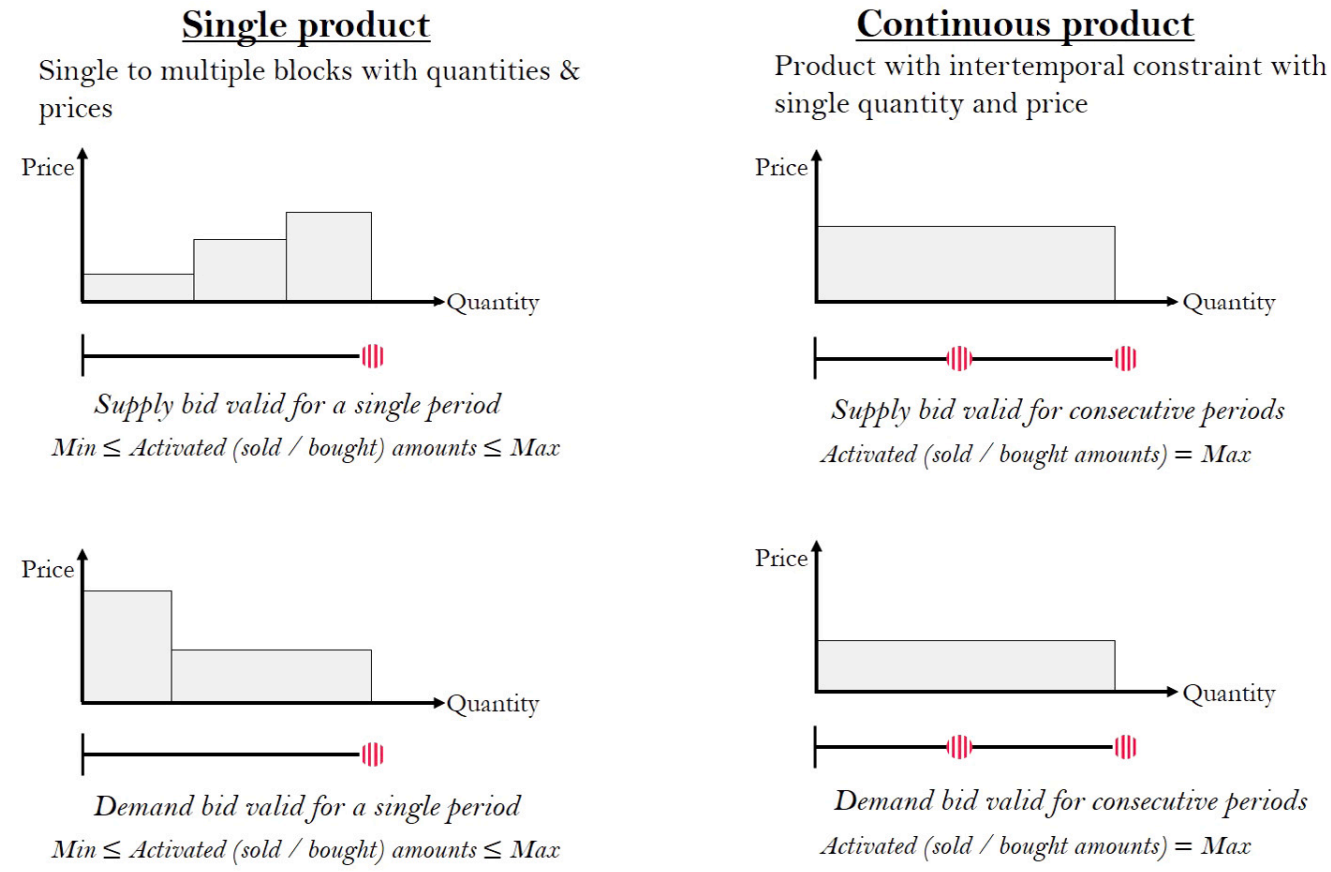
\includegraphics[scale=0.4]{Figures/DeMarket_Products.png}
    \caption{DeMarket Market Products \cite{DeTrade}}
\end{figure}

This market approach allows for many different type of bids and gives the opportunity to the peers to make more efficient trades. However, it becomes more difficult
to match the different bids efficiently. For this reason, $M$ marginal prices are calculated $P^x$, one for each delivery period $x$. The market model uses a uniform pricing mechanism
so on each delivery period $x$ the cost of energy is $P^x$ uniformly among the peers. These $M$ marginal prices are calculated based on a social welfare maximization problem, defined
by the summation of utility of all buyers minus the the summation of cost of all sellers, across all $M$ delivery periods. The authors of DeMarket, formulate the optimization equation
and uses the Ant-Colony optimization algorithm to calculate the mentioned prices $P^x$, in the clearing horizon steps $T_r = \{-R,\dots,-1\}$.
\cite{DeTrade}

\subsection{Blockchain Layer}
DeTrade uses a private and permissioned blockchain layer to achieve three main goals:
\begin{itemize}
    \item To store security the market clearing results
    \item To represent monetary value in the form of tokens (tokenization)
    \item And to automatically transfer digital tokens when the energy traded is actually delivered or consumed.
\end{itemize}
As it uses a private blockchain, a trusted third party (TTP) is needed which will be able to register new participants to the network and mint new tokens backed by real world currencies.
To achieve these goals, it defines the following smart contract methods:
\begin{table}[h!]
    \begin{tabular}{l|lll}
        Method                     & Scope   & Allowed Callers    & Description                               \\ \hline
        registerHousehold          & public  & TTP                & Add a new network peer                    \\
        mintEuroToken              & public  & TTP                & Add tokens on blockchain backed by Euro   \\
        balanceOf                  & public  & Smart Agents + TTP & Get the balance of a peer                 \\
        initializeRoles            & public  & Smart Agents       & Define the role (buyer/seller) of a peer  \\
                                   &         &                    & on each clearing horizon                  \\
        storeClearingResults       & public  & Smart Agents       & Store the clearing results after the      \\
                                   &         &                    & clearing horizon                          \\
        getTotalPrice              & public  & Smart Agents       & Returns the total cost of energy          \\
        receivedEnergy             & public  & Smart Agents       & Buyers invoke this method to confirm      \\
                                   &         &                    & energy is received and initiate the token \\
                                   &         &                    & exchange                                  \\
        isRegisteredHousehold      & private & -                  & Checks if a peer is already registered    \\
        resetClearingResults       & private & -                  & Resets the clearing results               \\
        validateAllClearingResults & private & -                  & Check if clearing results are valid       \\
        selectBestClearingResult   & private & -                  & Selects the best clearing result          \\
        redistributePoolFunds      & private & -                  & Moves the tokens between peers based on   \\
                                   &         &                    & delivery results
    \end{tabular}\\
    \rightline{\tiny Private methods cannot be invoked directly by a transaction}
    \caption{Smart Contract methods used by DeTrade.}
\end{table}
\\The blockchain technology used is Hyperledger Burrow which uses the BFT consensus algorithm and can tolerate up to $1/3$ of the participants being bad actors.
\cite{DeTrade}

\subsection{Limitations}
The two main limitation of this design are the following:
\begin{itemize}
    \item The assumption that prosumers report their real energy generation and that their forecast is error free. In reality, due
          to the irregularity of decentralized energy resources, the energy production forecasting is prone to errors. This leads to violations of energy trading
          commitments and the migrogrid is required to be connected to the grid in order to cover any extra energy needs at market cost.
    \item The strategic misreport of quantity and pricing bids. A peer could potentially try to manipulate the clearing price by placing strategic bids.
          Game theory could potentially help on creating a strategic-proof bidding process that is close to the optimal solution of the social welfare maximization
          problem.
\end{itemize}

\section{NRGCoin}
\label{sec:nrgc}
NRGCoin is a virtual currency backed by renewable energy production. It is a mechanism that facilitates the integration of renewable energy in the local grid
by making it more profitable for producers and utilities and cheaper for consumers and governments.
It allows local renewable energy producers to earn NRGcoins directly from their energy output, without depending on the market price or extra battery storage.
The NRGcoins can then be traded on an open market for their monetary equivalent at any time.\\
Information about the local energy production and consumption is sent every 15 minutes from the smart meters of the peers to the
street level low-voltage energy substation of the DSO. This information is used to determine the rates at which prosumers are rewarded with NRGCoins and
consumers are billed for energy withdrawal. These rates are determined buy the street-level substations that follows the NRGCoin protocol.
\cite{NRGCoin}

\begin{figure}[h!]
    \centering
    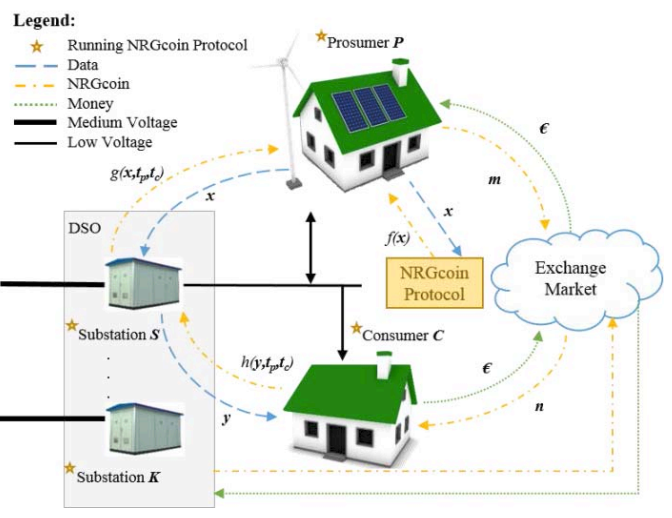
\includegraphics[scale=0.8]{Figures/nrgcoin.png}
    \caption{NRGCoin Schematic Setup \cite{NRGCoin}}
\end{figure}

\subsection{Market Layer}

NRGCoin is traded on an open currency exchange market. It can be traded openly between peers on the price they agree on. The price of the coin is influenced by
its value which is influenced by the rate at which coins are rewarded to prosumers for the energy they inject to the grid.
The NRGCoin network protocol is comprised by the following phases:
\begin{itemize}
    \item A prosumer $P$ generates $x$ amount of energy and broadcasts this information to the network
    \item The network peers are then updating the the public record of $P$ with $f(x)$ NRGCoins. $f()$ is the NRGCoin generation function that produces new
          NRGCoins that enters the circulation.
    \item The local substation $S$ which is connected to $P$ measures what is the total production $t_p$ and total consumption $t_c$ in
          that 15 minute slot.
    \item DSO transfers $g(x,t_p,t_c)$ NRGCoins to the balance of $P$. $g()$ is the production price function defined by DSO
    \item $P$ receives $f(x)$ NRGCoins from the NRGCoin protocol to ensure new money enters the system and $g(x,t_p,t_c)$ NRGCoins to motivate agents to match
          consumption with production.
    \item $P$ trades its acquired NRGCoins with a consumer $C$ based on their bids. The exchange can happen on any exchange platform with the NRGCoin listed
          each of which can potentially use different market clearing techniques.
    \item $C$ pays $h(y,t_p,t_c)$ NRGCoins to local substation $S'$ it's connected to, to consume $y$ amount of energy ($S$ and $S'$ could potentially be the same but it's not necessary).
\end{itemize}

The function $g(x,t_p,t_c)$ should be defined in a way to motivate the prosumers to produce energy based on the demand. Too much or too little energy production should result in lower
rewards in order to much demand. A bell curve reward function could motivate the prosumers to produce just enough energy:
\\
\begin{center}
    \begin{math}
        g(x,t_p,t_c) = \frac{x \times q}{e^\frac{(t_p-t_c)^2}{a}}
    \end{math}
\end{center}

Where $q$ is the maximum reward a prosumer can receive for their input energy $x$ when the total energy supply $t_p$ mather total demand $t_c$ and is defined by the DSO.
The parameter $a$ is used for scaling.\\
Function $h(y,t_p,t_c)$ is defined in a way to motivate the consumers to shift their consumption on times of high energy production. It is defined as:
\begin{center}
    \begin{math}
        h(x,t_p,t_c) = \frac{y \times r \times t_c}{t_c+t_p}
    \end{math}
\end{center}
Where $r$ is the maximum cost of energy defined by DSO, when energy supply is low ($t_p\rightarrow0$).
When $t_p >> t_c$, $h(x,t_p,t_c)\rightarrow0$ which means that in times of high production, energy is getting cheaper, incentivising consumers to consume at that times.

\subsection{Blockchain Layer}

NRGCoin is implemented as a network of hardware gateway devices interacting with the existing residential energy installation. They measure through sensors the energy
input and output and send these information regularly to the NRGCoin smart contract which implements the NRGCoin protocol. The smart contract can be either running on an
existing smart contract-capable public blockchain like Ethereum or on a network of the gateway devices supported by blockchain.
NRGCoin is deployed in reality on the Ethereum blockchain.
\cite{NRGCoin2}

\subsection{Limitations}
In this design we identify two main limitation:
\begin{itemize}
    \item The NRGCoin model is heavily depended on the current energy transfer installation. This creates a dependency to DSO and reduces the decentralization of the energy trading process
    \item Energy price can be manipulated by DSO
\end{itemize}

\section{Energy trading on CDA market}
\label{sec:cda}
This study proposes a model, leveraging blockchain and continuous double auctions. Buyers and sellers dynamically adapt prices within the auction to meet market fluctuations, with secure and 
transparent transactions recorded on the blockchain. In the following chapter, we describe in more details the market and blockchain layer of the proposed model and mention some of its possible 
limitations.

\subsection{Market Layer}
In this model, the CDA mechanism is used to clear the market bids. On each transaction period, prosumers and consumers submit their offering and asking bids to the network.
Based on the CDA mechanism the bids are matched and settled through the blockchain system. Unmatched peers adjust their bids according to a pricing strategy in order to find
a match. During the matching process, the market continuously discloses transaction information to the network peers, including transaction price, outstanding
bid and outstanding ask. These information can then be used to formulate a biding strategy.\\
When the final matching are done and settled through the blockchain, the energy producer receives the agreed payment through the blockchain and the consumer receives a digital
certificate of electricity transaction. The digital certificate of electricity transaction, gives the consumer the authorization to use the corresponding electricity.
\cite{wang2017novel}

\subsection{Blockchain Layer}
For this energy trading approach, the bitcoin protocol is used to settle the microgrid transaction. Consumers transfer bitcoin to the energy generators as a payment and the
energy generators transfer a special energy token as a digital certificate for the sale of electricity.
The transaction settlement process consists of the following steps:
\begin{itemize}
    \item The energy seller, issues a special energy token which is proportional to the transaction volume in the blockchain network.
    \item The seller sends a multi-signature redeemScript to consumer which contains the public key of the seller, the buyer and a trusted third party.
    \item The buyer creates a UTXO which has as an input the UTXO of the previous transaction and as an output the transfer of bitcoins to the given redeemScript along with
          a digital signature for verification.
    \item The seller creates a UTXO which has as an input the UTXO of the previous transaction and as an output the transfer of the special energy token to the public address of the buyer
          along with a digital signature for verification.
\end{itemize}
The multi-signature redeemScript is used to make sure that all both parties abide by their energy trade agreement. A trusted third party is also included in the multi-signature in order
to resolve any disputes between the parties. In case the seller doesn't transfer the special token to the buyer, the buyer doesn't sign the multi-signature transaction and the deal is rejected.
The trusted third party always signed the transaction except when there is a dispute between the parties at which case the transaction need to be investigated before resolving the transaction.\\
The special energy token issues by the sellers, prove the ownership of a certain amount of energy which can be transferred to an energy buyer to give them the permission to spend it.
In the bitcoin protocol, bitcoins are the only transaction object so in order to be able to have these special tokens in the network, special labels can be added to bitcoins to distinguish them from
common bitcoins. These specially labeled coins are called colored coins \cite{Colorcoin}.
\cite{wang2017novel}

\subsection{Limitations}
The main limitations we notices with this model are the following:
\begin{itemize}
    \item The CDA mechanism is not compatible with transactions that have inter-temporal commitments. This means that only energy needs of the next trading period can be covered
          and no energy trading planning for different time periods could be made.
    \item Prosumers might not be truthful about their hour ahead energy production or the forecasting might have some errors. This can lead to violations to the energy trading
          commitments. Such a system couldn't be self sustained, it needs to be connected to the grid to cover any extra energy needs.
    \item  Bitcoin might not be the best suit for this use case as it has a low block finality. of course the protocol could be adjusted on a private network to meet our needs
          where also a different consensus mechanism could be considered.
\end{itemize}

\section{Comparison}
\label{sec:comp}
Based on the reviewed literature, we can distinguish two different approaches to the energy trading problem.
One is the direct energy trading and the other is the pegging of a token to the energy value.
In the first approach, production and consumption forecasting is needed in order to match
energy trading needs of the peers while on the other an energy storage solution is needed.

\begin{table}[h!]
    \centering
    \begin{tabular}{l|llll}
        \textbf{Aspect}         & \textbf{\hyperref[sec:hfi]{A Frabric}}      & \textbf{\hyperref[sec:dtr]{DeTrade}} & \textbf{\hyperref[sec:nrgc]{NRGCoin}} & \textbf{\hyperref[sec:cda]{Energy trading}} \\
                                & \textbf{\hyperref[sec:hfi]{Implementation}} &                                      &                                       & \textbf{\hyperref[sec:cda]{on CDA market}}  \\
        \hline
        \textbf{Blockchain}     & Private                                     & Private                              & Public                                & Public                                      \\
                                & Hyperledger                                 & Hyperledger                          & Ethereum                              & Bitcoin                                     \\
                                & Fabric                                      & Burrow                               &                                       &                                             \\[5pt]
        \textbf{Consensus}      & BFT                                         & BFT                                  & PoS                                   & PoW                                         \\[5pt]
        \textbf{Market}         & MCP                                         & DeMarket                             & Open currency                         & CDA                                         \\
                                & (average buy offer)                         & pool-based                           & exchange                              &                                             \\[5pt]
        \textbf{Energy Trading} & Direct                                      & Direct                               & Indirect                              & Direct                                      \\
                                &                                             &                                      & Backed by MBRCoin                     &                                             \\[5pt]
    \end{tabular}
    \caption{Comparison of mentioned approaches}
\end{table}

\section{Summarization}
The investigated four distinctive models for decentralized energy trading, leveraging blockchain technology. We discussed about a private Hyperledger Fabric blockchain implementation that employs Byzantine Fault Tolerance (BFT) 
consensus for hourly direct energy trading, with limitations in inter-temporal commitments and potential forecasting inaccuracies. A private Hyperledger Burrow blockchain implementation called "DeTrade", focusing on direct energy 
trading with an emphasis on inter-temporal commitments. "NRGCoin" which follows a different energy trading paradigm, pegging a virtual currency to renewable energy production, though it faces limitations in reliance on existing 
energy transfer infrastructure. Finally, we also discussed about an energy trading implementation employing the CDA market mechanism. It uses Bitcoin protocol with the concept of colored coins to achieve direct energy trading but 
it is facing challenges with Bitcoin's low block finality. Each model offers distinct approaches to address decentralized energy trading complexities, with the choice contingent on factors like decentralization preference and 
specific energy market requirements.